\section{What is drone racing?}

As in any race, competitors measure their skills at maneuvering their vehicle,
from within or at distance, against the clock or against themselves, in an
attempt to complete a circuit before everyone else.

In drone racing, the circuit is comprised of a set of obstacles, static or
dynamic, usually arranged in a loop. For the case of classic drone racing, huge
futuristic-looking arenas are used as a playground for extremely skilled pilots,
who make the race look impressive and dynamic by the use of FPV goggles to fly
the drones at very high speed, reaching 120mph
\cite{https://thedroneracingleague.com/learn-more/}.

\begin{figure}[h]
	\centering
	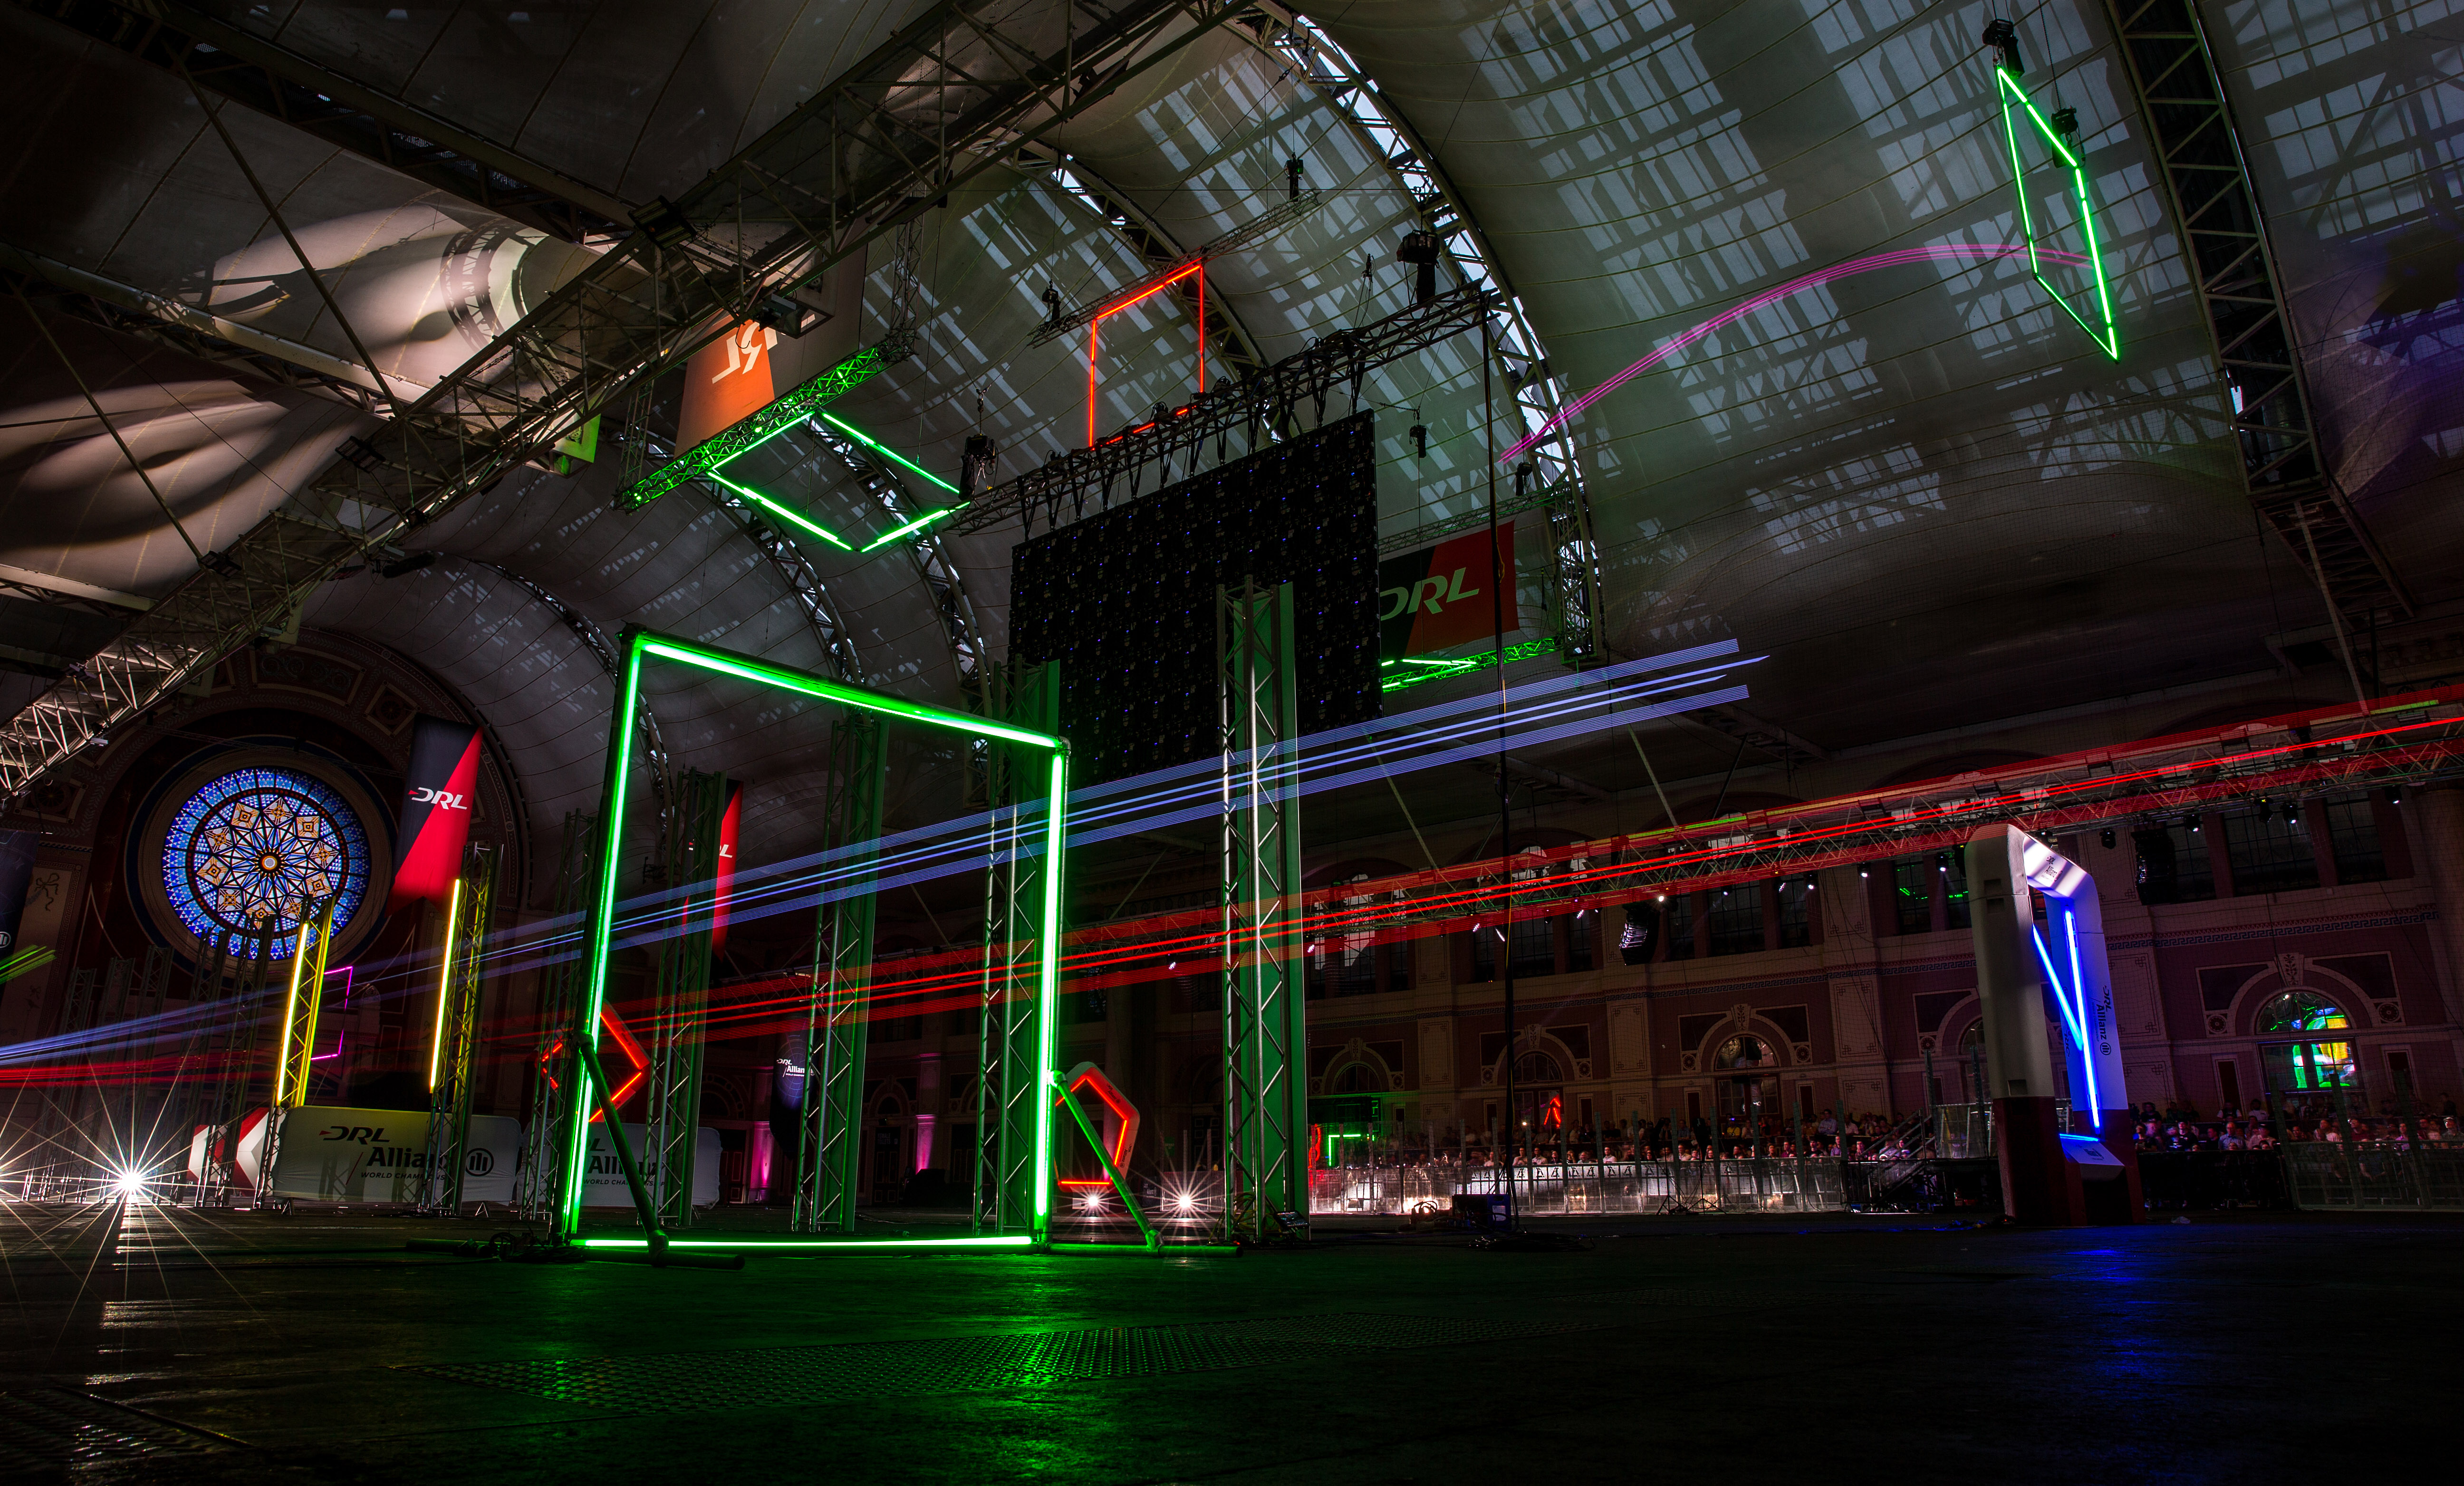
\includegraphics[width=0.5\textwidth]{figure/drl_arena.jpg}
	\caption{Drone Racing League arena in London (Steven Paston/PA)}
\end{figure}

\todo{cite image https://home.bt.com/tech-gadgets/tech-news/the-drone-racing-league-has-set-a-new-world-record-for-the-fastest-drone-around-11364196881110}
	
For the case of autonomous drone racing, up until the \emph{Drone Racing
League} announced their autonomous competition of 2019, arenas looked much more
like a laboratory than a glowing circuit, as it can be seen on Figure
~\ref{fig:mygates} showing the AiR Lab in Skejby (Aarhus, DK), with its gates
built and painted for this work. These obstacles were inspired of the previous
competitions organized by IROS, as seen on Figure ~\ref{fig:iros} which also
shows the typical type of drones used in this research area: consumer drones
for the larger audience. This kind of drones is not made for sportive flight,
but mostly for an easy hands-on experience, providing a relatively slow but
stable flight.

\begin{figure}[h]
	\centering
	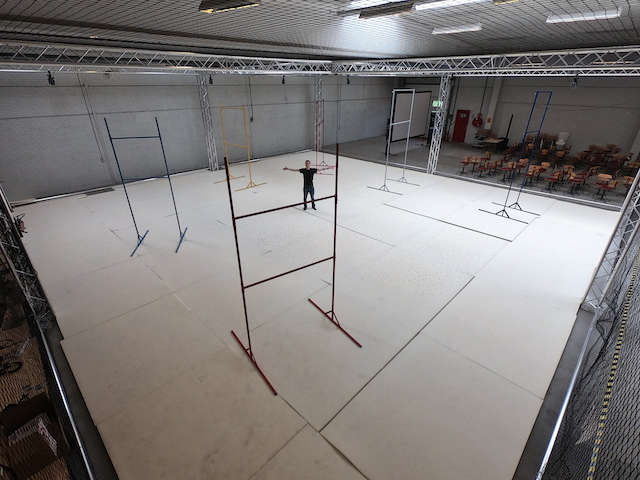
\includegraphics[width=0.5\textwidth]{figure/tiny_me.jpg}
	\caption{The AiR Lab and the custom built obstacles around the author in Skejby}
	\label{fig:mygates}
\end{figure}

The goal is to complete a given amount of turns as fast as possible, but since
it is still the early days of drone racing and the costs of a potential crash
would be too high, each drone races against the clock, one after an other.
Ultimately, autonomous drones will be racing against skilled pilots, as the
\emph{Drone Racing League} seems to encourage it by giving a total prize of 2
millions USD for the race of 2019.


\subsection{Stakes}
\todo{Talk about the predictions for AI in drone racing and drones in general
for the future}


\subsection{Beyond the hype and into reality}
\todo{Talk about Amazon Prime Air, food delivery, driverless taxis...}


\subsection{Challenges}
Most robotic system's operation can be modeled by the commonly known
\emph{Sense, Plan, Act} paradigm:
\todo{Add custom act, sense, plan paradigm picture}
\begin{figure}[h]
	\centering
	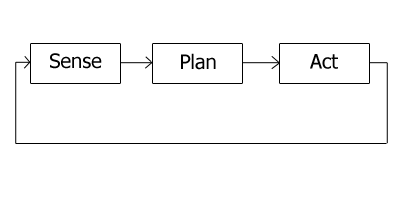
\includegraphics[width=0.4\textwidth]{figure/robotic_paradigm.png}
	\caption{The Sense, Plan, Act robotic paradigm.}
	\label{fig:robotic_paradigm}
\end{figure}

\begin{itemize}
	\item{\textbf{Sense}}: gather information using sensors (camera, IMU, sonar...).
	\item{\textbf{Plan}}:create a world model using all the information, and plan
		the nextmove.
	\item{\textbf{Act}}: carry out the actions that the plan calls for.
\end{itemize}
~\\
This thesis will be focused mainly on the sensing of the drone control, and
more precisely using computer vision algorithms along with machine learning
concepts. However, an important part of the trajectory planning directly
follows the sensing phase, therefore those two first phases of the control loop
can be included in the scope of the project.

To this day, most drones in the robotic research field are running \emph{Robot
Operating System} (ROS) \todo{Add citation}, which is a set of "libraries and
tools to help software developers create robot applications". The implementation
of the computer vision algorithms will be constrained within ROS, and cooperate
with the different control components provided by the project team.\\



